\section{Phase 2: Low Fidelity Prototype}
\subsection{Methodology}
We used the results from our preliminary survey to design two sketch-based low fidelity prototypes of an AR system containing aspects of in-store and online shopping experiences that participants identified as important.  We can bring critical factors of online experiences, such as access to reviews and ease of comparison, into the store environment while preserving aspects of in-store decision making, such as being ``hands-on with the product'' and leaving the store with the product. We hypothesized that an augmented reality application that supplemented a traditional in-store experience with immediate access to core aspects of online shopping would improve consumer's confidence in their purchasing decisions. \todo{replace the last bit of this sentence with what was actually tested}

\todo[inline]{JRB: The paragraph below talks about one prototype. I think you should say that you had two. One prototype for interaction concept.}
We tested our hypothesis in a think-aloud study using our sketch-based prototypes as a design prompt. \todo{JRB: Formative design work and evaluation do not have to be hypothesis driven, and often aren't. Instead they are exploratory. If you are feeling encumbered by the "hypothesis" language, we can reword. Just let me know.} The prototypes, shown in figures \ref{fig:LowFiContext} and \ref{fig:LowFiMenu} consisted of online content drawn as AR menus on transparency sheets and overlaid onto an image of an electronics store. Participants were tasked with choosing a laptop to purchase in each prototype, with the first prototype to be tested chosen randomly for each participant. We used the two prototypes to make a comparison between a menu-based, hierarchically structured user experience, and a context-aware virtual overlays of product information. \todo{what specific AR components were tested here (e.g., reviews, product comparisons, specs, etc.)? What were your measures here (e.g., confidence in the decision, time to decision, etc.)} \todo{JRB: How did you analyze the data from this phase?}
\todo[inline]{figure of paper prototype}

\begin{figure}
	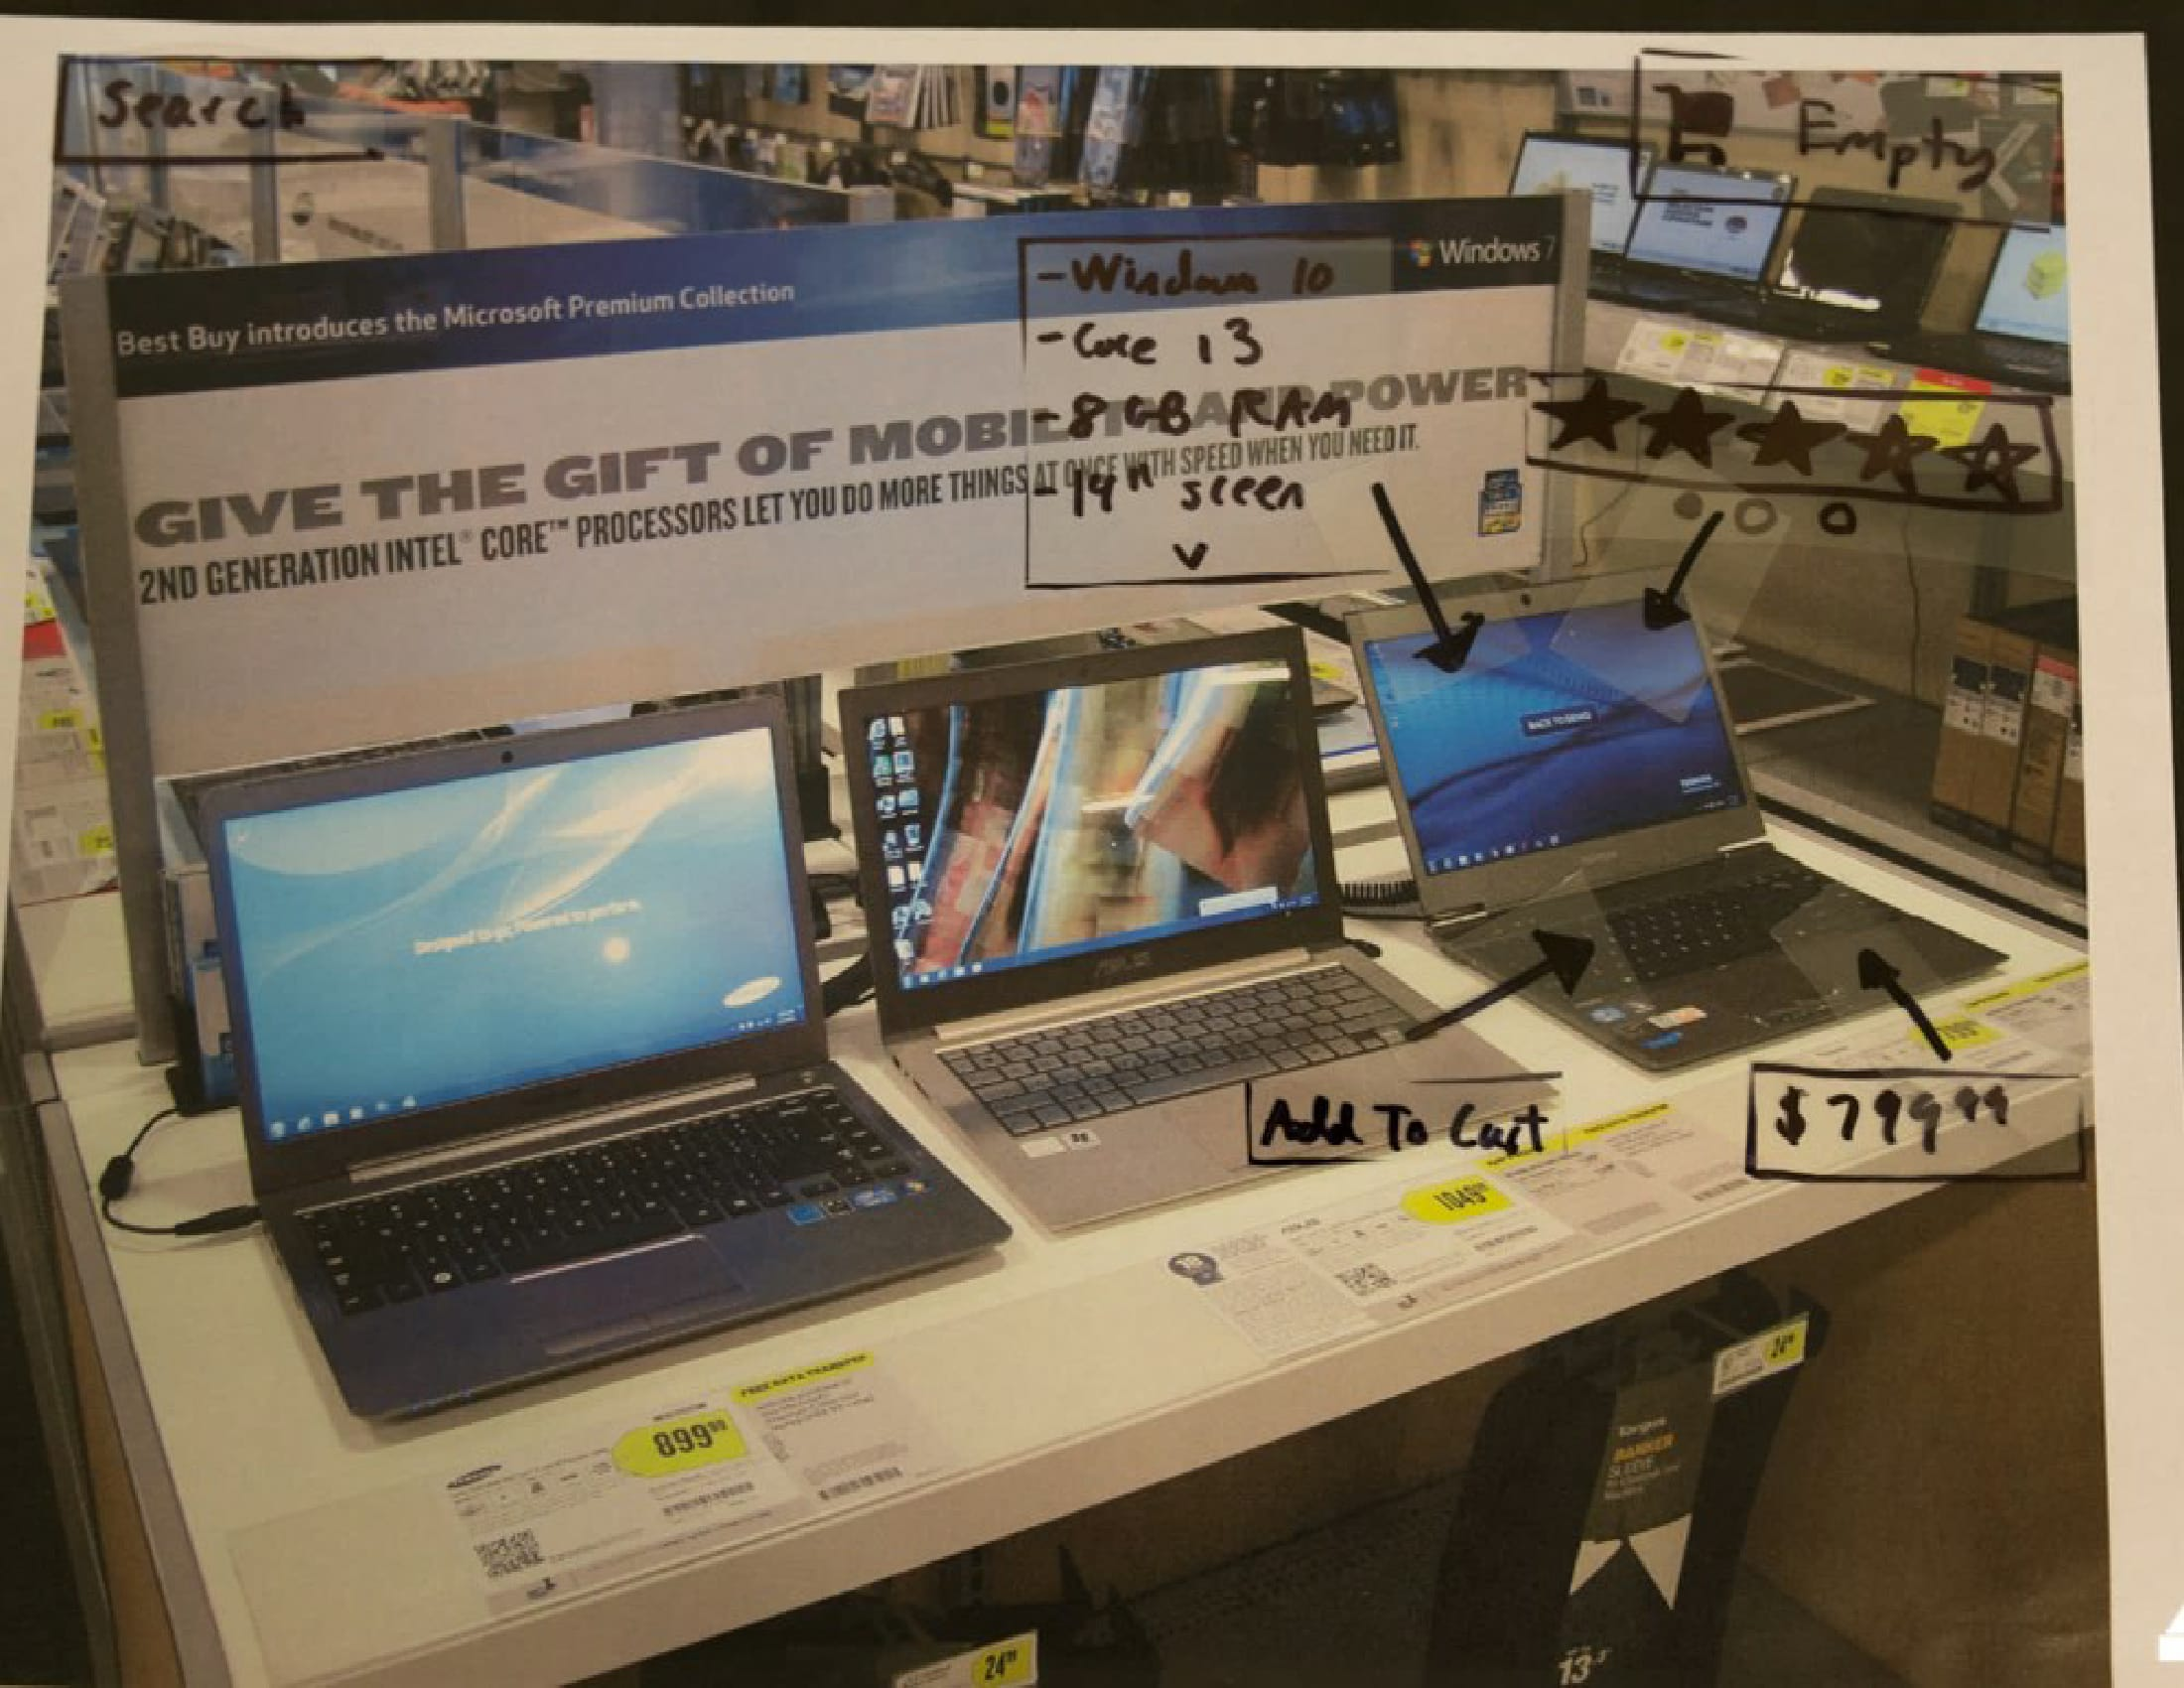
\includegraphics[width=0.9\columnwidth]{figures/LowFiContext}
	\caption{Context-aware paper prototype}
	\label{fig:LowFiContext}
\end{figure}
\begin{figure}
	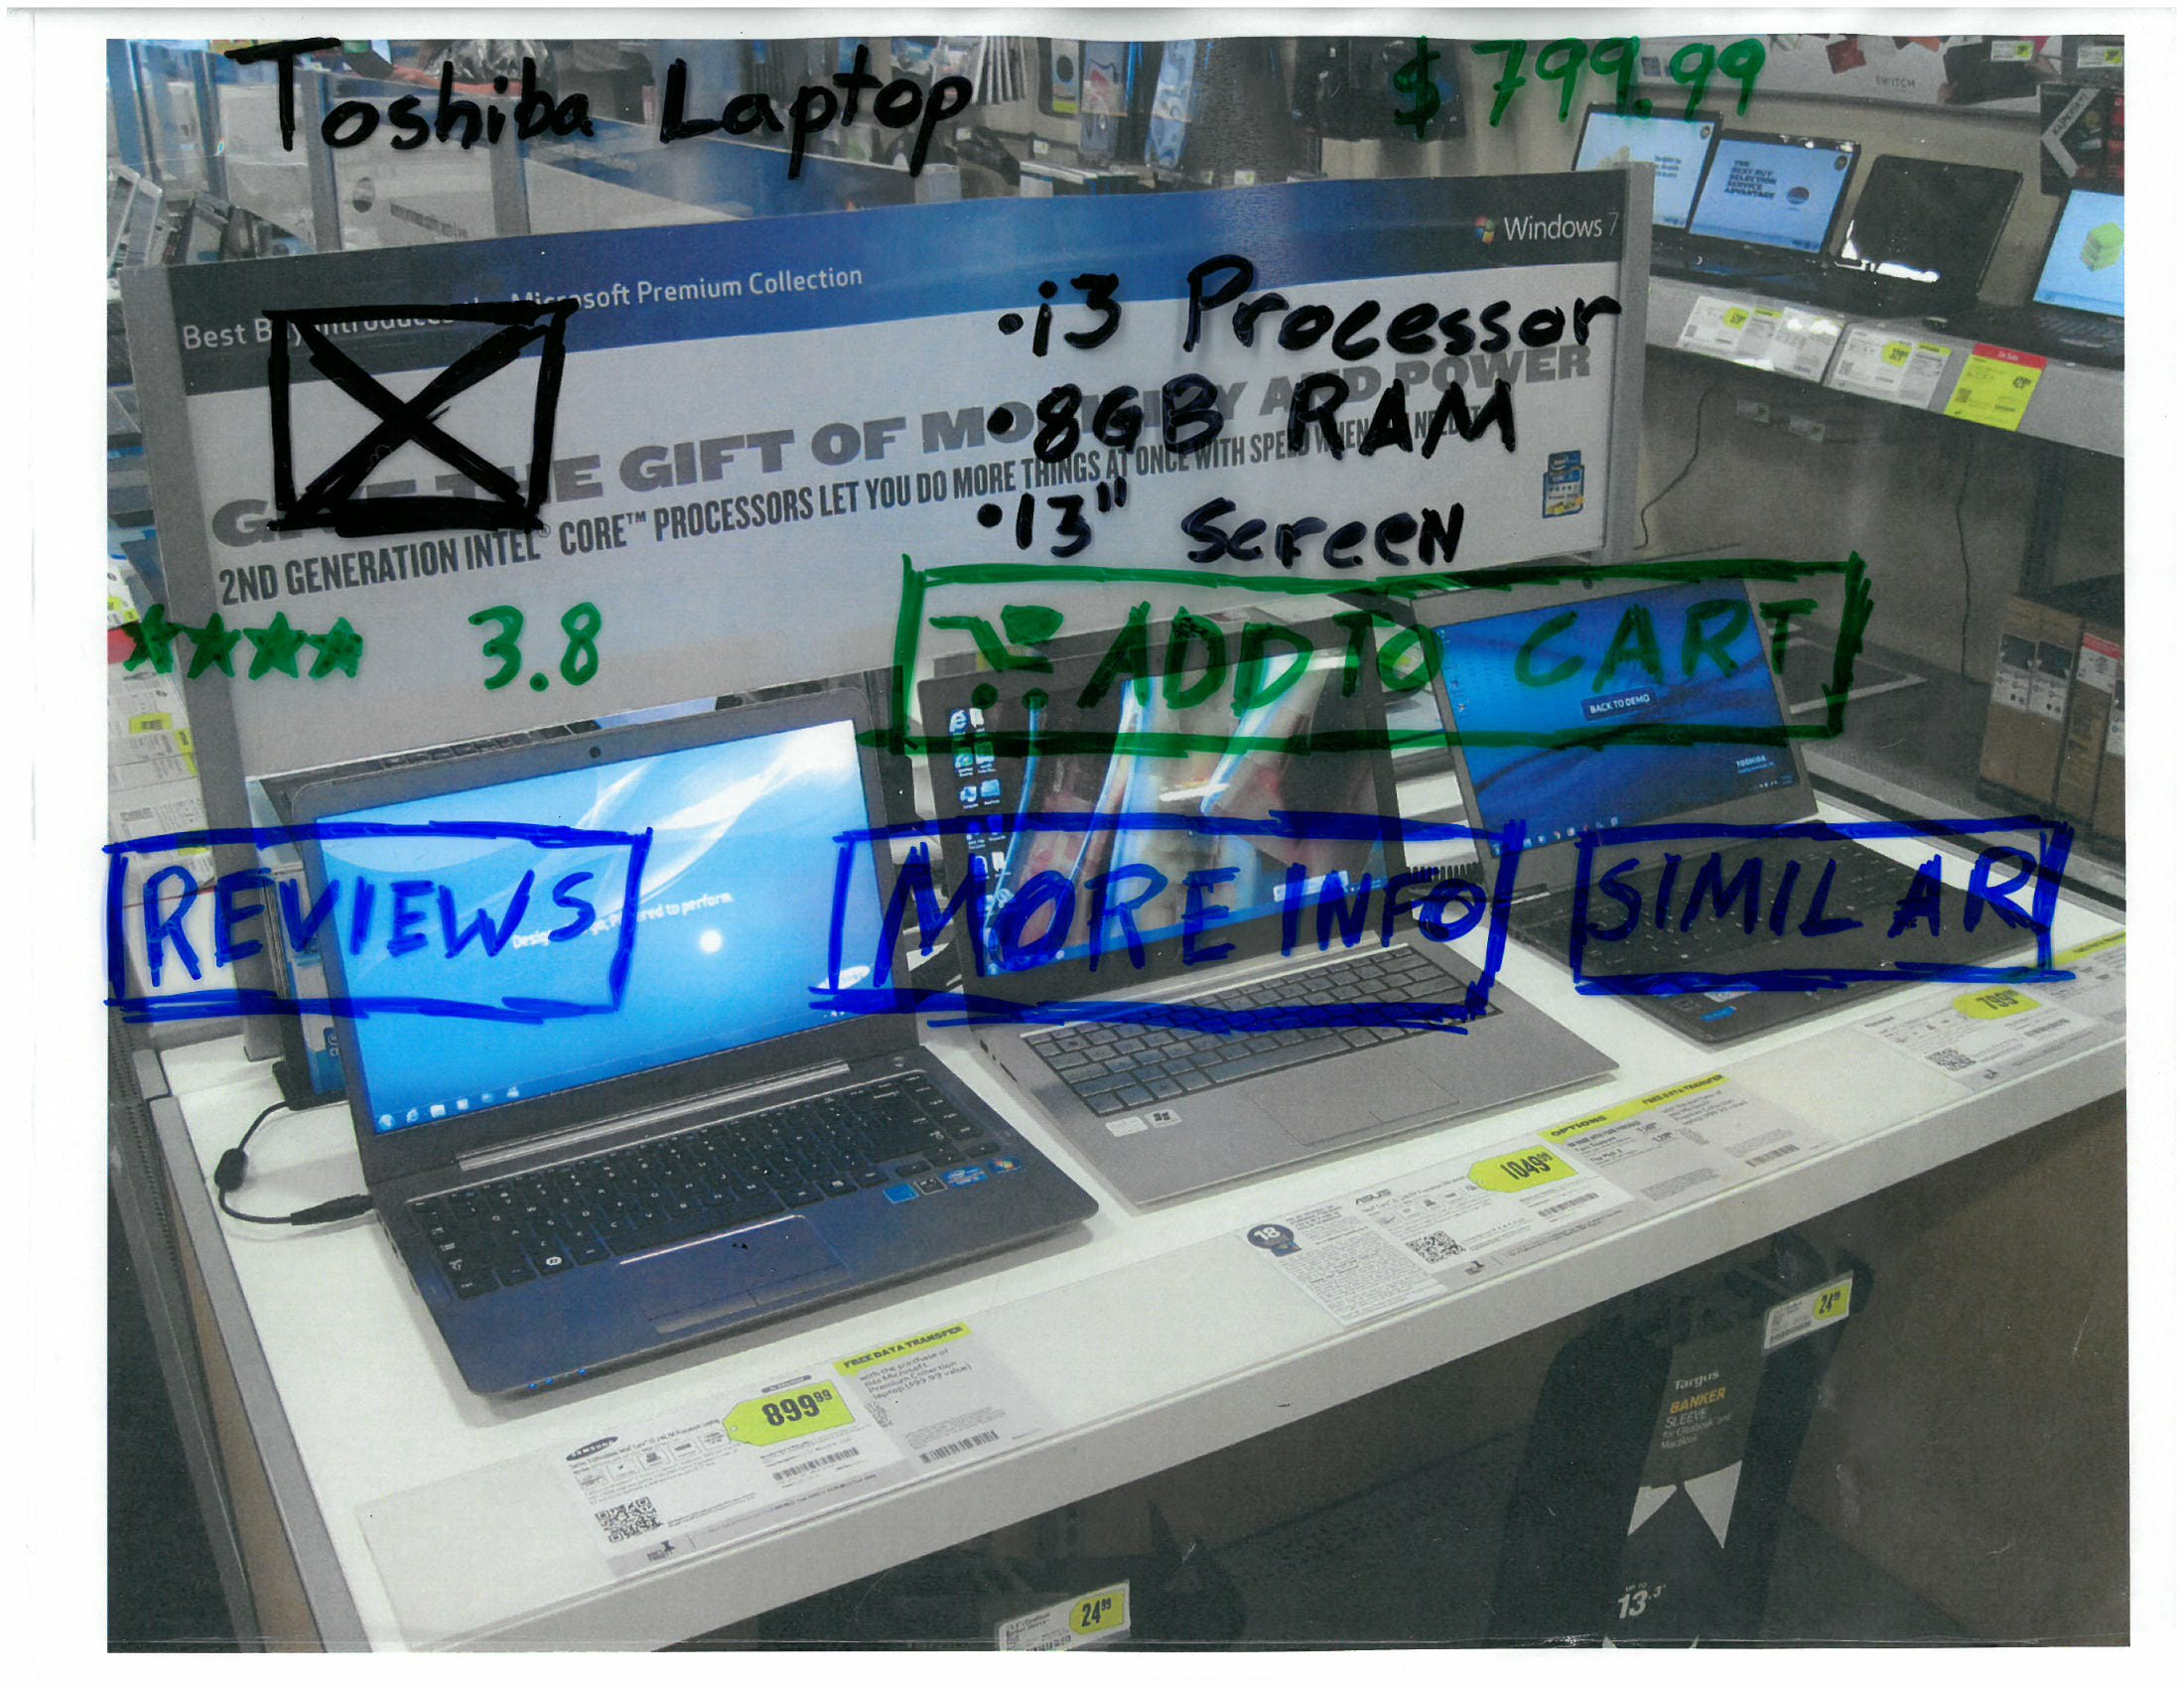
\includegraphics[width=0.9\columnwidth]{figures/LowFiMenu}
	\caption{Menu-based paper prototype}
	\label{fig:LowFiMenu}
\end{figure}

\subsection{Findings}
We recruited three participants from campus for this study. Generally, participants were more receptive to quick and less information than to the fuller, menu-based approach. Participants stated that the ability to compare the specifications of two different laptops in the same view is valuable in decision-making. Participants also expressed a desire to toggle display of content. One participant identified demos as a useful application of augmented reality in retail.